\documentclass{report}

\usepackage[utf8]{inputenc} % Charakter-Kodierung
\usepackage[german]{babel} % Sprache

\usepackage[table,xcdraw]{xcolor} % Tabellen Farben
\usepackage{tabularx} % Dynamische Tabellenbreite
\usepackage{tcolorbox} % Graue Boxen
\usepackage{hyperref} % url Umgebung
\usepackage{todonotes} % Notizen
\usepackage{natbib} % Bibliographie
\usepackage{fancyhdr} % Header und Footer
\usepackage{multirow} % Multizeile
\usepackage{geometry} % Page layout
\usepackage{color} % Text Farben

\usepackage[hashEnumerators,smartEllipses]{markdown}

% Page layout
\geometry{
	bottom=3.5cm,
	headheight=180pt
}

% Nummerierung der ersten Seiten verhindern
\pagenumbering{gobble}

% Bibstyle
\bibliographystyle{plain}

% Header / Footer
\fancypagestyle{plain}{
	\fancyhf{}% Clear header/footer
	\fancyhead[R]{
\includegraphics[width=4cm]{img/cau-logo-2017}} % Rechter header
	\fancyhead[L]{\leftmark} % Linker header
	\fancyfoot[R]{\thepage} % Rechter footer
	\fancyfoot[L]{
\includegraphics[width=1cm]{img/se-logo}} % Linker footer	
}
\pagestyle{plain}

\renewcommand{\headrulewidth}{0.5pt} % Unnötige Informationen der Kapitelangabe
\renewcommand{\footrulewidth}{0.2pt} % entfernen
\renewcommand{\chaptermark}[1]{\markboth{{#1}}{}}




% Zahlen für Fußnoten
\renewcommand{\thefootnote}{\arabic{footnote}}
\renewcommand{\thempfootnote}{\arabic{mpfootnote}}

%%%%% Ausfüllen %%%%%

% Gruppenname
\newcommand{\gruppenname}{Gruppe LMS8 EG 016}

% Projektname
\newcommand{\projektname}{VOTEsso}

% Semester
\newcommand{\semester}{Sommer 2022}



% Titelseite

\title{
	\vspace*{-5cm}
	Pflichtenheft\\
	\textbf \projektname\\
	Bürgerbeteiligung Kiel\\
	-\\
	\color{gray}
	Softwareprojekt \semester\\
	\gruppenname\\
	\vspace*{5mm}
	
\includegraphics[width=\textwidth]{img/logo}
}

\author{
	\begin{tabular}{r l@{\hspace{8\tabcolsep}} r} 
		Heiko & Bielfeldt & \multirow{8}{*}{ 
\includegraphics{img/se-logo} } \\
		Markus & Glaubitz \\
		Niclas & Nebelung \\
		Sören & Petersen \\
		Arne & Seufert \\
		Jonas & Struve \\
		Jon & Stührwoldt \\
		Arne & Wiese \\
	\end{tabular}
}

\date{\today}


% Dokument

\begin{document}
	\maketitle
	
	\tableofcontents
	
	\chapter{Lizenz}\label{chp:lizenz}
	\pagenumbering{arabic} % Nummerierung starten
	
\textbf{Copyright	2022}\\\\
Heiko Bielfeldt, Markus Glaubitz, Arne Wiese, Jonas Struve, Sören Petersen, Jon Stührwoldt, Niclas Nebelung und Arne Seufert\\
Licensed	under	the	Apache	License,	Version	2.0	(the	”License”);	you	may	not	use	this	file	except	in
compliance	with	the	License.	You	may	obtain	a copy of	the	License	at\\
\begin{verbatim}
http://www.apache.org/licenses/LICENSE-2.0
\end{verbatim}
Unless	required	by	applicable	law	or	agreed	to	in	writing,	software	distributed	under	the	License	is
distributed	on	an	“AS	IS”	BASIS,	WITHOUT	WARRANTIES	OR	CONDITIONS	OF	ANY	KIND,	either	express
or	implied.	See	the	License	for	the	specific	language	governing	permissions	and	limitations	under	the
License.
	
	\chapter{Produkteinsatz}\label{chp:produkteinsatz}
	

\begin{markdown}

## Zielgruppen

Das Produkt soll für AuA jeden Alters ohne weiterführende (technische) Vorkenntnisse - die über die Verwendung eines Appfähigen Geräts, die Installation einer App oder Bedienung eines Web-Browsers hinausführen - geeignet sein.

Da AuA Teil der Projektergebnisse sein könnten, wird eine hohe Partizipation in der Webanwendung und App erwartet. Diese Beteiligung ermöglicht dem Projektleiter zusätzliche Informationen der potentiellen Anwenderinnen und Anwender einzuholen, welche sich potentiell positiv auf die Qualität der Projekte auswirken können.

Neben den geringfügigen technischen Vorkenntnissen, sollen die AuA jedwige Information über Projekte problemlos finden. Daher wird auch sichergestellt werden, dass die Bedienung der Webanwendung und App leicht verständlich ist, damit die AuA die Nutzung der Webanwendung und App maximieren und eine Vielzahl von etwaigen wichtigen aber noch unbekannten Informationen mitteilen.

In Achtung des digitalen Zeitgeistes wird eine intensivere Nutzung der App erwartet. Infolgedessen kann die Endfassung der App mehr Funktionen bereitstellen als die Webanwendung. AuA werden auf ihren Wegen im Alltag mobile Geräte benutzen und sollen dabei durch eine schneller und unkomplizitere Öffnung der App (im Vergleich zur Webanwendung) unterstützt werden. Dennoch sollen AuA mit geringfügiger Präferenz appfähige Geräte zu benutzen die Möglichkeit erhalten Projektinformationen einzusehen.
\end{markdown}
\newpage

\begin{markdown}
## Anwendungsgebiete

AuA in den Planungs- und Umsetzungsprozess eines Projekts integrieren. "Integrieren" der AuA in jeden Prozess ist dabei wie folgt definiert:

1. Aktuelle Informationen zum entsprechenden Projekt und zugehörigen Teilprojekten bereitstellen. Transparenz des Projektvorgangs soll die Außenwirkung des Projekts positiv beeinflussen und die Anzahl von AuA erhöhen.
2. Soziale Involvierung von AuA durch individuelle Meinungsverbreitung in Form von Kommentaren zu (Teil-)Projekten. AuA sollen angeregt werden über Teile von Projekten zu diskutieren und so auch eine umfassendere und reflektierte Meinung zu entsprechenden Themen aufzubauen, die den Projektprozess unterstützen und die Qualität des Endprodukt des Projekts steigern könnten.
3. Alle Projektinformationen werden dauerhaft verfügbar sein, um eine barrierefreie Nutzung der App oder Webanwendung zu gewährleisten. Somit sind Projektinformationen zu jeder Zeit und an jedem Ort spontan verfügbar.
\end{markdown}

	
	\chapter{Zielbestimmungen}\label{chp:zielbestimmungen}
	Im Folgenden werden Notationen "i)", "ii)", "iii)" und "iv)" verwendet, die zur semantischen Zuordnung von Informationen über die Arten der Kriterien hinaus dienen sollen. Die Bedeutung der Notation sei wie folgt definiert:\\\\

\begin{tabularx}{\textwidth}{X X}
		\rowcolor[HTML]{C0C0C0}
		\textbf{Notation} & \textbf{Bedeutung} \\
		i) & Kriterien für die Startseite\\
		\rowcolor[HTML]{E7E7E7} 
		ii) & Kriterien für die Seite eines Hauptprojekts\\
		iii) & Kriterien für die Seite eines Teilprojekts\\
		\rowcolor[HTML]{E7E7E7} 
		iv) & Kriterien für den allgemeinen Datenbestand\\
\end{tabularx}

\begin{markdown}
  
Des Weiteren werden die Kriterien (soweit notwendig) zur App und/oder zur Webanwendung zugeteilt.

## Muss-Kriterien

**App & Webanwendung**

i) Startseite

* Präsentation aller Hauptprojekte mit Weiterleitungsmöglichkeit zum jeweiligen Inhalt

ii) Hauptprojekt

* Darbietung aktualisierter Informationen des Hauptprojekts
* Auflistung aller zugehörigen Teilprojekte mit Weiterleitungsmöglichkeit zur Inhaltsübersicht
* Ordnung von Teilprojekt-Liste nach geodatenbasierter Relevanz
* Es wird ein Zurück-Button bereitgestellt, welcher den Anwender zur Startseite zurückführt

iii) Teilprojekt

* Darbietung aktualisierter Informationen des Teilprojekts
* Implementierung von einem Zurück-Button, welcher den Anwender zur Seite des übergeordneten Hauptprojekts zurückleitet
* Kommentare von AuA zu einem Teilprojekt sind für alle AuA sichtbar

iv) Datenbestand

* Die App und die Webanwendung teilen sich denselben Datenbestand, der nach jeder Änderung von Projektinhalten und Verfassen von Kommentaren aktualisiert wird
* Verbal-geschriebene bzw. textuelle Informationen werden in der deutschen Sprache dargeboten
* Für die Erstanwendung der App und Webanwendung werden notwendige Standardwerte in Hinsicht der Netzwerkadressierung automatisch implementiert

**App**

i) Startseite

* AuA erhalten die Möglichkeit Netzwerkadressen und Ports der App-Anwendung der Hintergrunddienste zu spezifizieren

iii) Teilprojekt

* AuA haben die Möglichkeit einen Kommentar zum Teilprojekt zu verfassen

**Webanwendung**

i) Startseite

* Weiterleitungsmöglichkeit zur Login-Seite für Admins
* Admins können Kommentare löschen
* Der Admin kann die notwendigen Netzwerkadressen und Ports von Consul und der zugehörigen Datenbank über eine Maske in der Webanwendung manuell einstellen

## Soll-Kriterien

**App und Webanwendung**

ii) Hauptprojekt

* Einbettung von Informationen über den Fortschritt und die Planung des Hauptprojekts

iii) Teilprojekt

* AuA können Teilprojekte bewerten. Dafür wird es die Möglichkeit zu einer positiven oder negativen Bewertung geben.

**App**

iii) Teilprojekt

* Geodatenbasierte Anzeige der Stadtkarte inklusive Stecknadeln der zugehörigen Teilprojekte

## Kann-Kriterien

**App und Webanwendung**

i) Startseite

* Weiterleitung zur Detailseite der Hauptprojekte über Pinnadeln auf einer Karte

ii) Hauptprojekt

* Zusätzliche Weiterleitungsmöglichkeit zur Detailseite eines Teilprojekts über die Stecknadeln auf der Stadtkarte
* AuA können das Hauptprojekt kommentieren und bewerten
* AuA können eigene Kommentare löschen und bearbeiten

iii) Teilprojekt

* AuA können eigene Kommentare löschen und/oder bearbeiten

iv) Datenbestand

* AuA können sich registrieren, anmelden und abmelden.
* Anzeige der durchschnittlichen Bewertung von einem ii) Hauptprojekt oder iii) Teilprojekt
* Verbal-geschriebene bzw. textuelle Informationen werden in mehreren Sprachen angeboten
\end{markdown}
\newpage

\begin{markdown}
## Abgrenzungskriterien

**App und Webanwendung**

* In der App und Webanwendung wird keine Funktion bereitgestellt die die Einbindung der Kamera benötigt
* Auf Kommentare kann nicht geantwortet werden
* AuA können nicht abstimmen, ob ein Hauptprojekt durchgeführt werden soll und es werden auch keine Alternativen zum jeweiligen Hauptprojekt angeboten
* AuA werden nicht geprüft, ob sie in Kiel gemeldet sind

## Sonstiges

* In Achtung der vom Kunden gesetzten Rahmenbedingung wird für die Umsetzung der Anwendungen die Programmiersprache Java verwendet
\end{markdown}
	
	\chapter{Produktfunktionen}\label{chp:produktfunktionen}
	\begin{figure}[h]
	\centering
	
	\begin{tabularx}{\textwidth}{ p{.2\textwidth} | X | X }
		\textbf{Akteur} & \textbf{Beschreibung} & \textbf{Verwendet in Anwendungsfall} \\ \hline
		Nutzer & Bei Nutzern handelt es sich um die Anwender
 der Webanwendung und der App. Hierbei ist keine Authentifizierung erforderlich. Nutzer können sich auf
 den beiden Nutzeroberflächen mittels Verlinkungen zwischen den Haupt- und Teilprojekten bewegen.
 In der Android-App kann ein Nutzer zusätzlich zum reinen Lesen (read-only in Webanwendung) noch
 Teilprojekte bewerten und Kommentare verfassen. & A01, A02, A03, A04 \\ \hline
		Administrator & Der Administrator hat zusätzlich zu den Berechtigungen des Nutzers
 die Möglichkeit, von der Webanwendung aus, Kommentare zu löschen. Das admin-Konto ist dabei vorgegeben
 und die Verwaltung von Benutzeraccounts gehört damit nicht zu den Aufgaben dieses Administrators. & W01, W02
	\end{tabularx}

	
	\caption{Beschreibung der Akteure}
	\label{fig:akteur-tabelle}
\end{figure}


%%%%%%%%%%%%%%%
%% Anwendungsfall 1 %%
%%%%%%%%%%%%%%%
\newpage
\section{Anwendungsfalldiagramme}
Die Anwendungsfalldiagramme haben den Zweck, die Kernfunktionen der Software fur die verschiedenen Akteure zu beschreiben.
\subsection{Anwendungsfalldiagramm - App}

\begin{figure}[h]
	\centering
	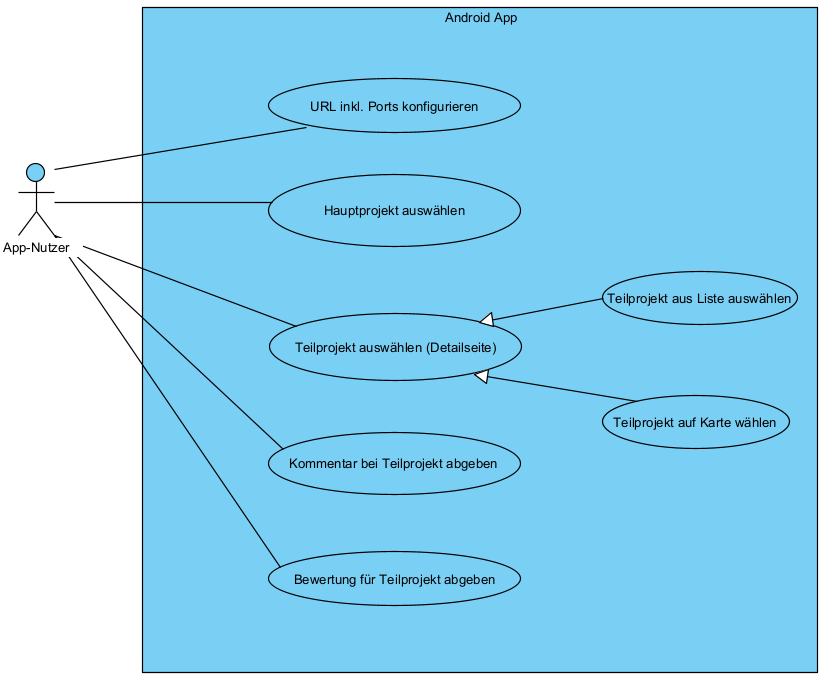
\includegraphics[width=\textwidth]{img/usecaseandroid.png}		
	\caption{Anwendungsfalldiagramm - App}
	\label{fig:anwendungsfalldiagramm-app}
\end{figure}

\newpage

\newpage

%%%%%%%%%%%%%%%
%% Anwendungsfall 2 %%
%%%%%%%%%%%%%%%
\newpage

\subsection{Anwendungsfalldiagramm - Webanwendung}

\begin{figure}[h]
	\centering
	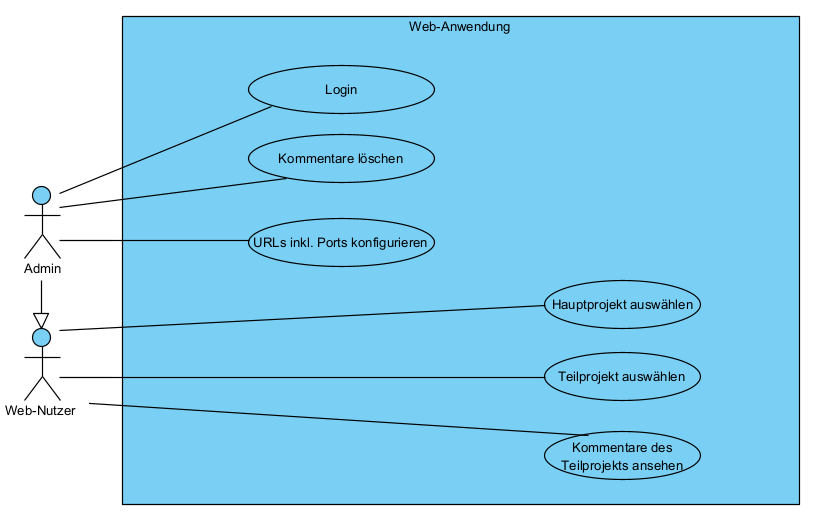
\includegraphics[width=\textwidth]{img/usecaseweb.png}	
	\caption{Anwendungsfalldiagramm - Webanwendung}
	\label{fig:anwendungsfalldiagramm-server}
\end{figure}

\newpage

\section{Anwendungsfälle}
Im Folgendem sind die wichtigsten Anwendungsfälle aufgelistet. Unterstützend stehen Mockups zur Verfügung, um einen Eindruck von der geplanten grafischen Oberfläche zu geben.
\begin{figure}[h]
	\centering
	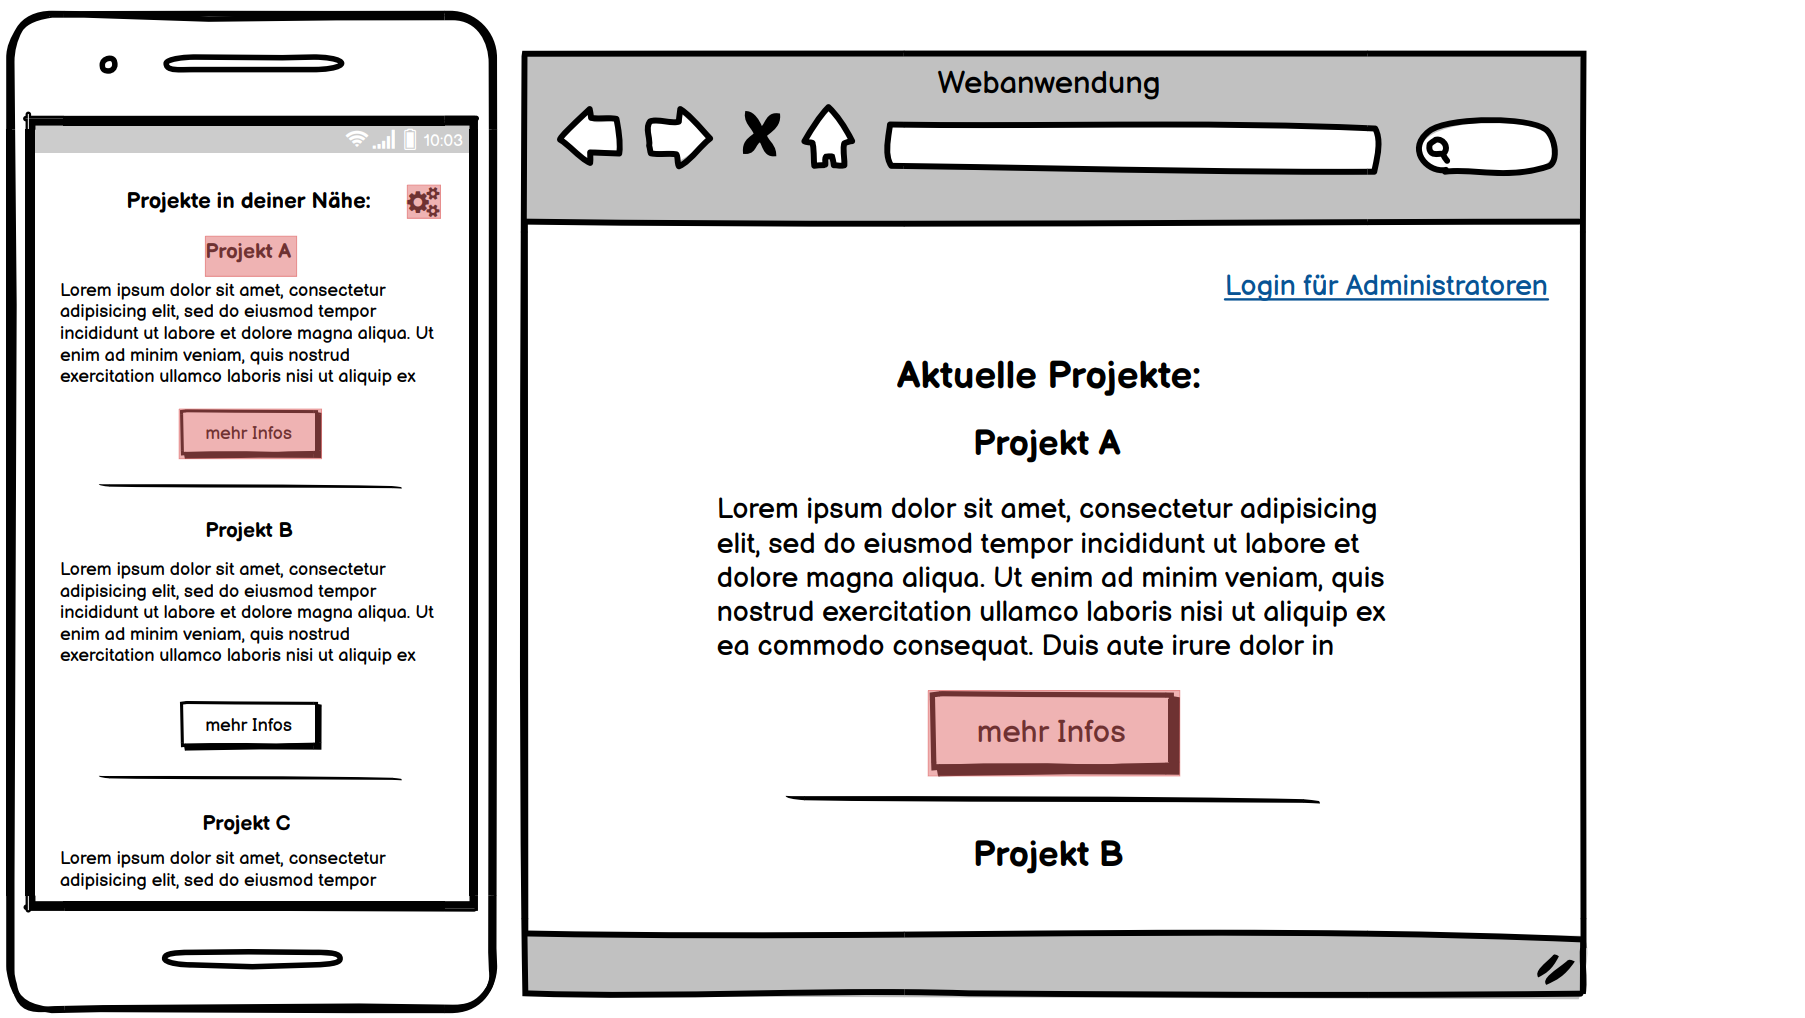
\includegraphics[width=\textwidth]{img/MUstart.png}			
	\caption{Startseite}
	\label{fig:anwendungsfalldiagramm-app}
\end{figure}

\begin{figure}[h]
	\centering
	\begin{tabularx}{\textwidth}{ X | X }
		\textbf{Anwendungsfall ID} & A01 \\ \hline
		\textbf{Anwendungsfallname} & Teilprojekt auswählen (Detailseite) (App, Webanwendung) \\ \hline
		\textbf{Initiierender Akteur} & Nutzer \\ \hline
		\textbf{Kurzbeschreibung} & Der Nutzer wählt ein spezifisches Teilprojekt des jeweiligen Hauptprojektes.  \\ \hline
		\textbf{Vorbedingungen} & Der Nutzer befindet sich auf der Seite eines Hauptprojektes.  \\ \hline
		\textbf{Nachbedingungen} & Der Nutzer befindet sich auf der Detailseite des ausgewählten Teilprojektes.  \\ \hline
		\textbf{Ablauf} &
			\begin{enumerate}
				\item Der Nutzer sucht auf der Seite eines Hauptprojekt ein Teilprojekt aus der nach Entfernung sortierten Liste aus.
				\item Der Nutzer tippt auf das gewünschte Teilprojekt.
			\end{enumerate} \\ \hline
		\textbf{Alternative} &
				\begin{enumerate}
					\item  Der Nutzer wählt das gewünschte Teilprojekt, indem er auf eine Stecknadel auf der eingebetteten Karte tippt.
				\end{enumerate}  \\ \hline
		\textbf{Ausnahme} &
				\begin{enumerate}
					\item Das Hauptprojekt enthält keine Informationen über Teilprojekte.
				\end{enumerate}  \\ \hline
	\end{tabularx}
	\caption{Anwendungsfall A01}
	\label{fig:anwendungsfall-app-tabelle-xx-1}
\end{figure}

\begin{figure}[h]
	\centering
	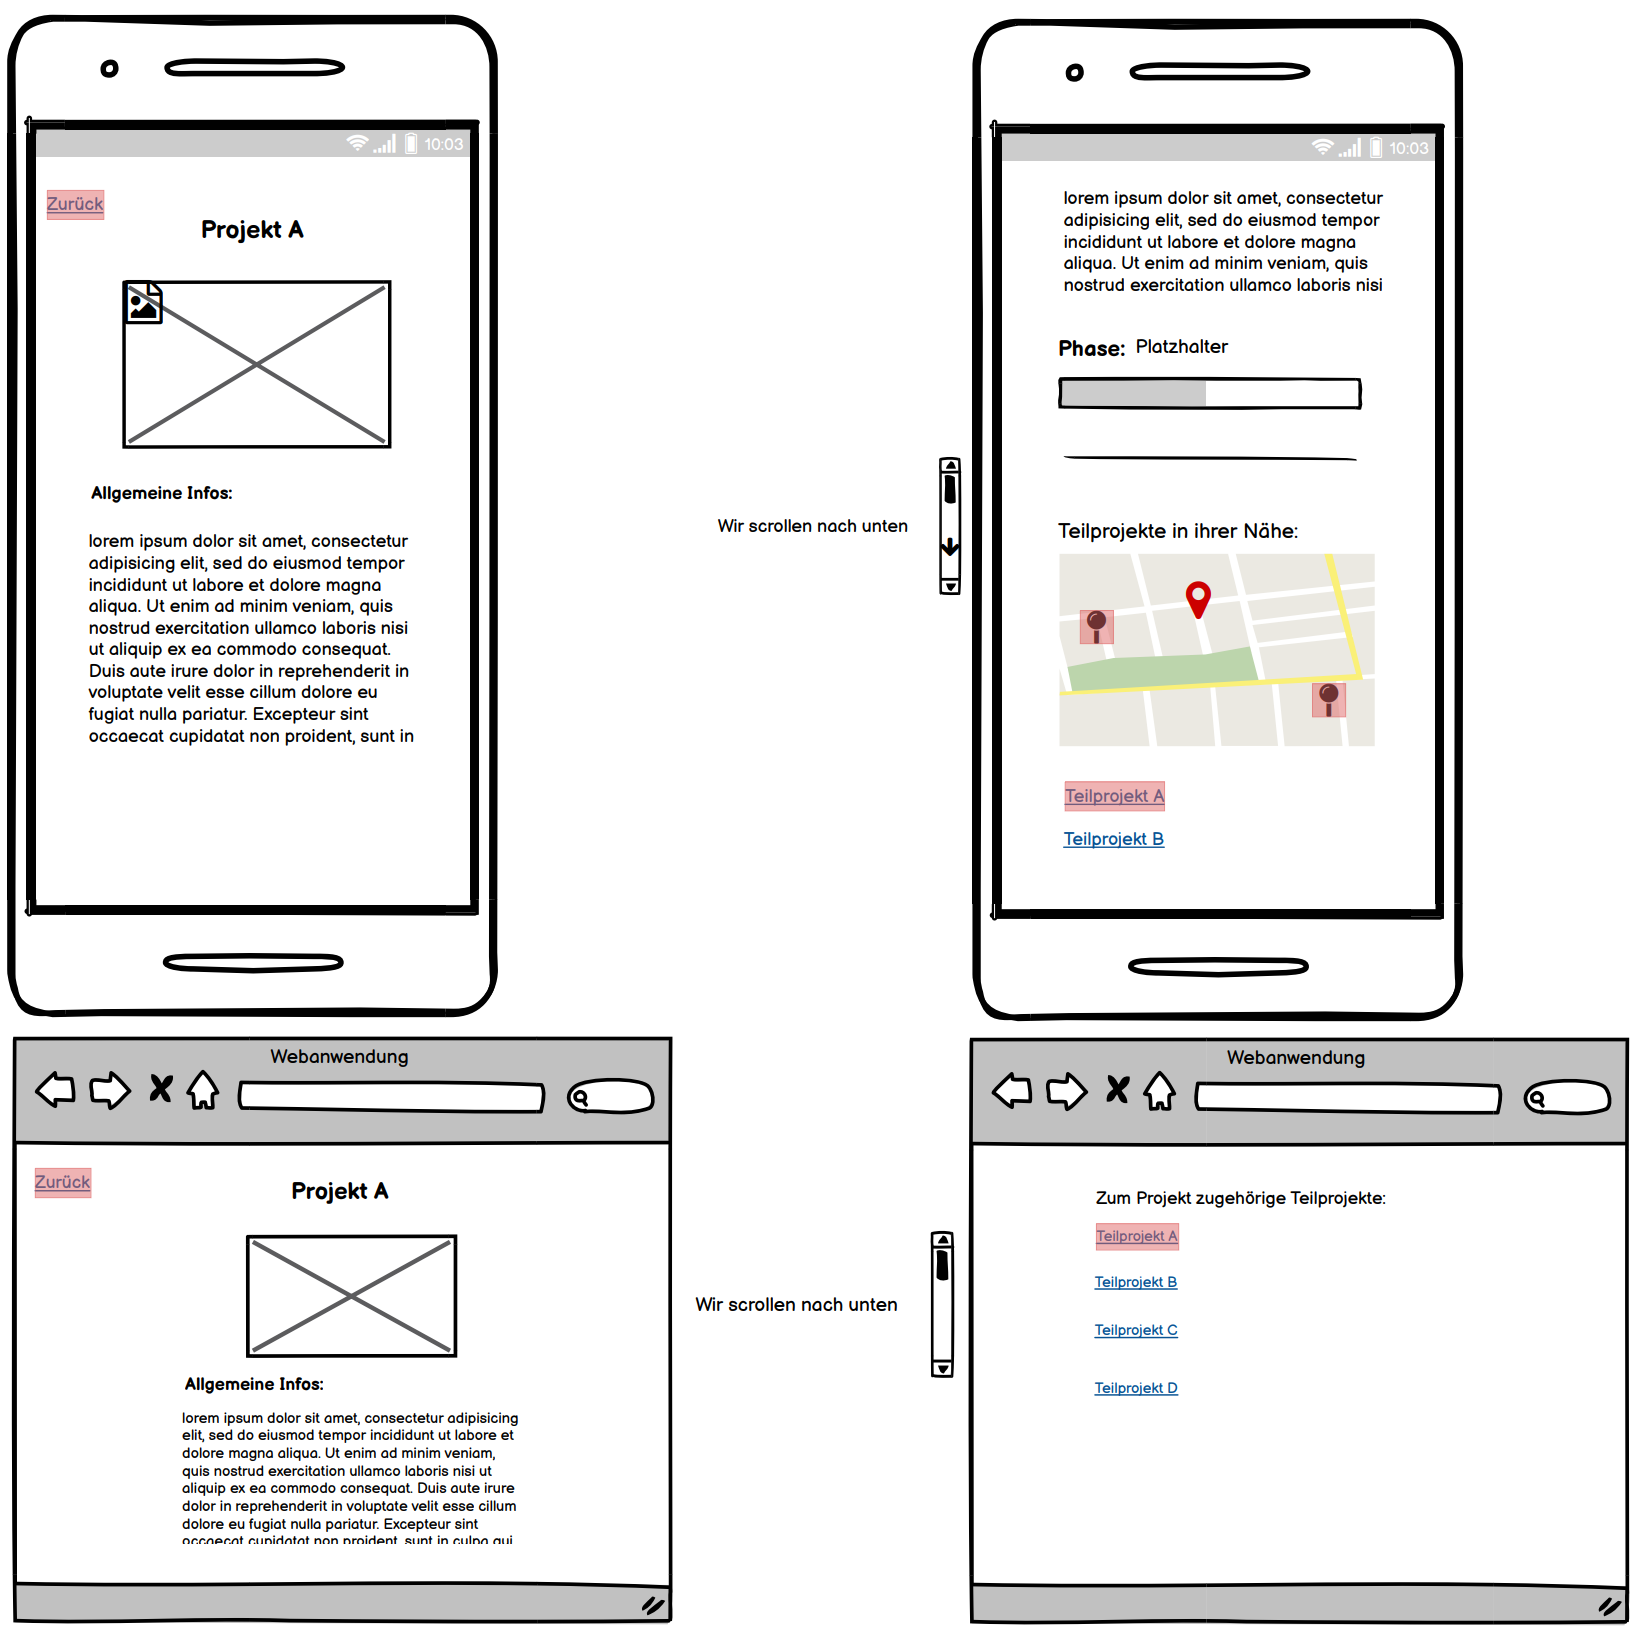
\includegraphics[width=\textwidth]{img/MUhaupt.png}			
	\caption{Auswahl Teilprojekt}
	\label{fig:anwendungsfalldiagramm-app}
\end{figure}


\begin{figure}[h]
	\centering
	\begin{tabularx}{\textwidth}{ X | X }
		\textbf{Anwendungsfall ID} & A02 \\ \hline
		\textbf{Anwendungsfallname} & Kommentar bei Teilprojekt abgeben (App) \\ \hline
		\textbf{Initiierender Akteur} & Nutzer \\ \hline
		\textbf{Kurzbeschreibung} & Der Nutzer gibt einen schriftlichen Kommentar zu einem Teilprojekt ab  \\ \hline
		\textbf{Vorbedingungen} & Der Nutzer befindet sich auf der Detailseite eines Teilprojektes  \\ \hline
		\textbf{Nachbedingungen} & Der Kommentar wird in der öffentlichen Kommentarsektion des Teilprojektes angezeigt, Der Nutzer erhält eine Bestätigung über die Abgabe seines Kommentars.  \\ \hline
		\textbf{Ablauf} &
			\begin{enumerate}
				\item Der Nutzer tippt in das Kommentarfeld und gibt seinen Kommentar ein.
				\item Der Nutzer tippt auf den Button "Absenden".
			\end{enumerate} \\ \hline
		
	\end{tabularx}
	\caption{Anwendungsfall A02}
	\label{fig:anwendungsfall-app-tabelle-xx-1}
\end{figure}

\begin{figure}[h]
	\centering
	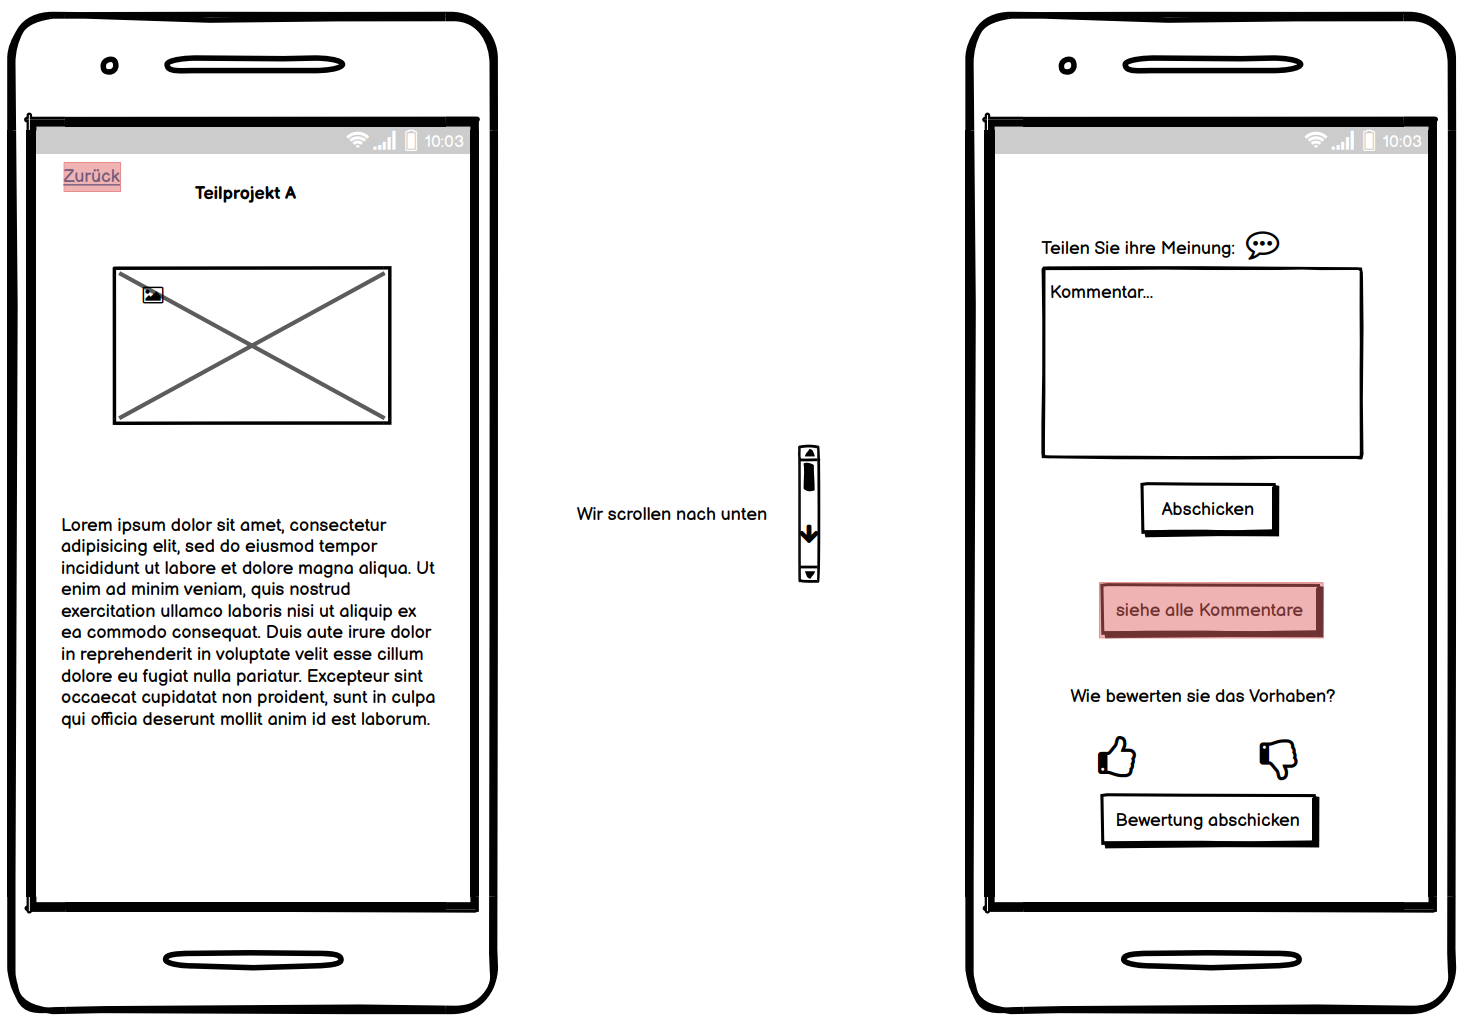
\includegraphics[width=\textwidth]{img/MUcomment.png}			
	\caption{Teilprojekt kommentieren und bewerten}
	\label{fig:anwendungsfalldiagramm-app}
\end{figure}

\begin{figure}[h]
	\centering
	\begin{tabularx}{\textwidth}{ X | X }
		\textbf{Anwendungsfall ID} & A03 \\ \hline
		\textbf{Anwendungsfallname} & Bewertung abgeben (App) \\ \hline
		\textbf{Initiierender Akteur} & Nutzer \\ \hline
		\textbf{Kurzbeschreibung} & Der Nutzer bewertet ein Teilprojekt mittels Daumen.  \\ \hline
		\textbf{Vorbedingungen} & Der Nutzer befindet sich auf der Detailseite eines Teilprojektes.  \\ \hline
		\textbf{Nachbedingungen} & Eine Bestätigung für die Abgabe der Bewertung wird angezeigt (evtl. mit farblicher Hinterlegung des jeweiligen Daumens).  \\ \hline
		\textbf{Ablauf} &
			\begin{enumerate}
				\item Der Nutzer tippt auf den gewünschten Daumen.
			\end{enumerate} \\ \hline
	\end{tabularx}
	\caption{Anwendungsfall A03}
	\label{fig:anwendungsfall-app-tabelle-xx-1}
\end{figure}


\begin{figure}[h]
	\centering
	\begin{tabularx}{\textwidth}{ X | X }
		\textbf{Anwendungsfall ID} & A04 \\ \hline
		\textbf{Anwendungsfallname} & URL inklusive Ports konfigurieren (App) \\ \hline
		\textbf{Initiierender Akteur} & Nutzer \\ \hline
		\textbf{Kurzbeschreibung} & Der Nutzer ändert die URL des Backend-Servers.  \\ \hline
		\textbf{Vorbedingungen} & Der Nutzer befindet sich auf der Einstellungsseite.  \\ \hline
		\textbf{Nachbedingungen} & Ein Bestätigungstext wird angezeigt.  \\ \hline
		\textbf{Ablauf} &
			\begin{enumerate}
				\item Der Nutzer gibt gewünschte URL in das Textfeld ein.
				\item Der Nutzer bestätigt die neue URL indem er auf den Button „Bestätigen“ tippt.
			\end{enumerate} \\ \hline
	\end{tabularx}
	\caption{Anwendungsfall A04}
	\label{fig:anwendungsfall-app-tabelle-xx-1}
\end{figure}

\begin{figure}[h]
	\centering
	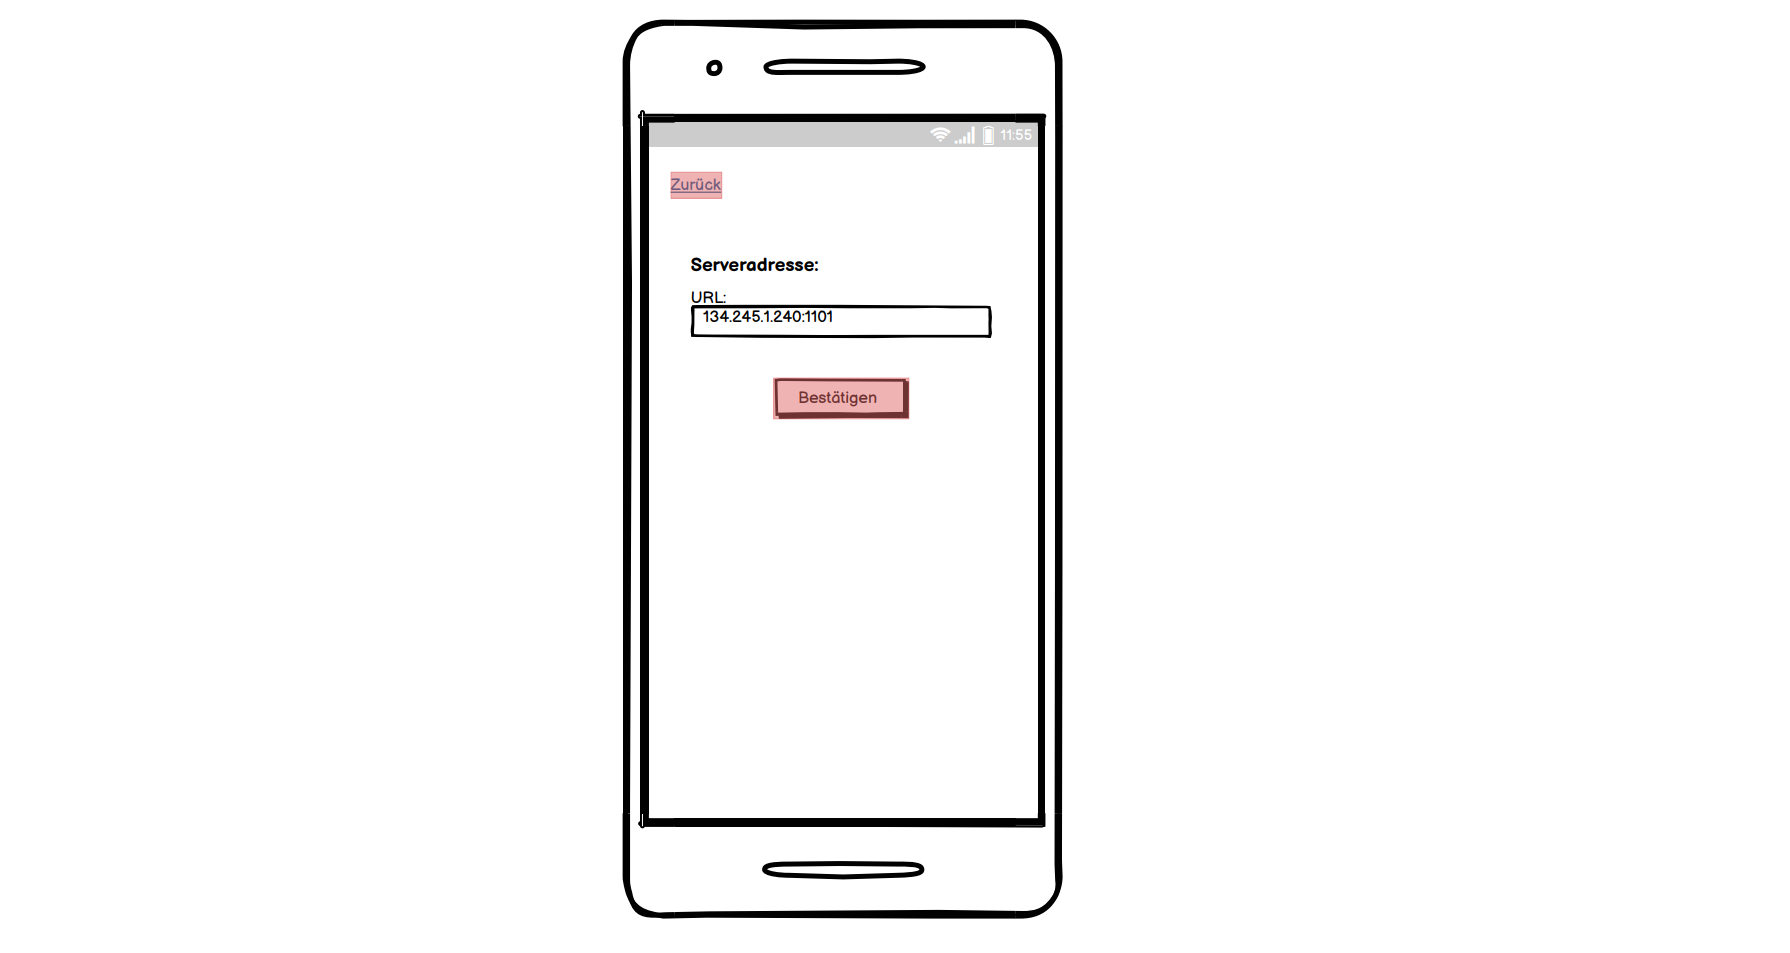
\includegraphics[width=\textwidth]{img/MUurl.png}			
	\caption{URL konfigurieren}
	\label{fig:anwendungsfalldiagramm-app}
\end{figure}


\begin{figure}[h]
	\centering
	\begin{tabularx}{\textwidth}{ X | X }
		\textbf{Anwendungsfall ID} & W01 \\ \hline
		\textbf{Anwendungsfallname} & Kommentar löschen (Detailseite) (App, Webanwendung) \\ \hline
		\textbf{Initiierender Akteur} & Administrator\\ \hline
		\textbf{Kurzbeschreibung} & Der Administrator löscht den gewünschten Kommentar.  \\ \hline
		\textbf{Vorbedingungen} & Der Administrator ist als Benutzer admin eingeloggt. Der Administrator befindet sich auf der Detailseite eines Teilprojektes.  \\ \hline
		\textbf{Nachbedingungen} & Der Text des Kommentars wurde geändert auf „Dieser Kommentar wurde vom Administrator gelöscht.“.  \\ \hline
		\textbf{Ablauf} &
			\begin{enumerate}
				\item Der Administrator wählt Kommentar aus, welcher gelöscht werden soll.
				\item Der Administrator löscht den Inhalt des Kommentars, indem er auf den Button "Löschen" tippt.
			\end{enumerate} \\ \hline
	\end{tabularx}
	\caption{Anwendungsfall W01}
	\label{fig:anwendungsfall-app-tabelle-xx-1}
\end{figure}

\begin{figure}[h]
	\centering
	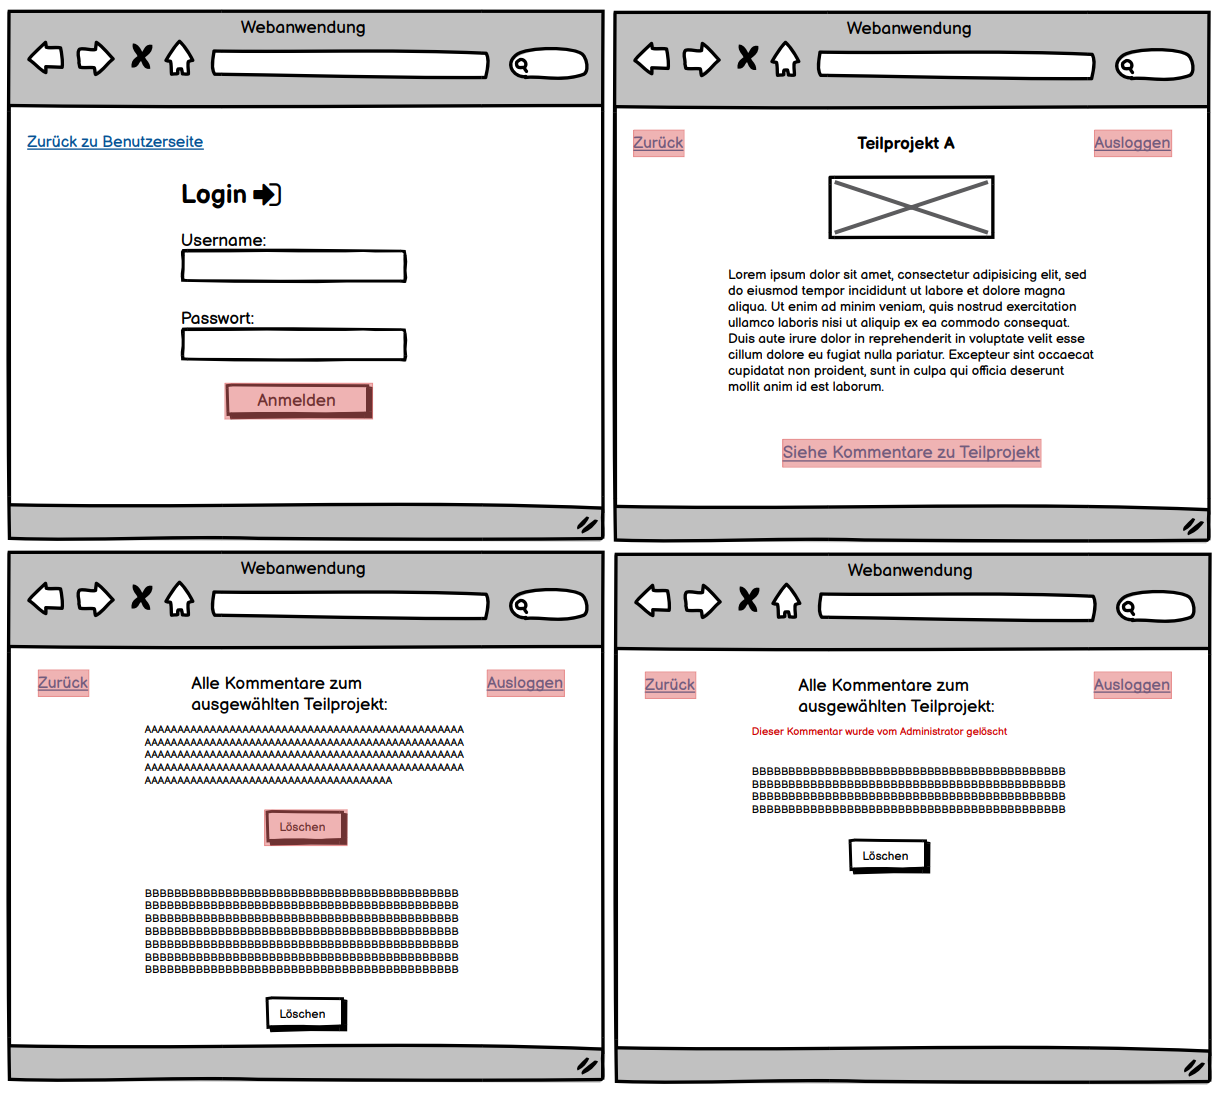
\includegraphics[width=\textwidth]{img/MUdelete.png}			
	\caption{Kommentar löschen}
	\label{fig:anwendungsfalldiagramm-app}
\end{figure}


\begin{figure}[h]
	\centering
	\begin{tabularx}{\textwidth}{ X | X }
		\textbf{Anwendungsfall ID} & W02 \\ \hline
		\textbf{Anwendungsfallname} & URLs inklusive Ports konfigurieren (Webanwendung) \\ \hline
		\textbf{Initiierender Akteur} & Administrator\\ \hline
		\textbf{Kurzbeschreibung} & Der Administrator ändert die URLs der Anwendung für die Datenbank und/oder das Backend  \\ \hline
		\textbf{Vorbedingungen} & Der Administrator ist als Benutzer admin eingeloggt. Der Administrator befindet sich auf der Einstellungsseite.  \\ \hline
		\textbf{Nachbedingungen} & Ein Bestätigungstext wird angezeigt.  \\ \hline
		\textbf{Ablauf} &
			\begin{enumerate}
				\item Der Administrator gibt die gewünschte URL in das jeweilige Textfeld.
				\item Der Administrator bestätigt die neue URL mit einem Klick auf den Button „Bestätigen“.
			\end{enumerate} \\ \hline
	\end{tabularx}
	\caption{Anwendungsfall W02}
	\label{fig:anwendungsfall-app-tabelle-xx-1}
\end{figure}

\begin{figure}[h]
	\centering
	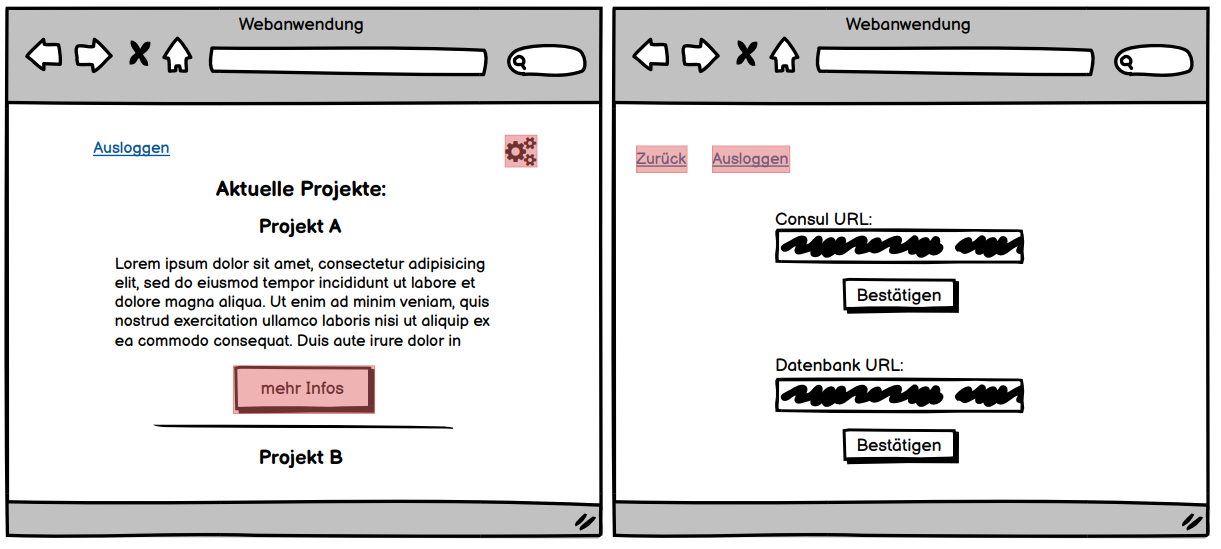
\includegraphics[width=\textwidth]{img/MUurlweb.png}			
	\caption{Backend URL konfigurieren}
	\label{fig:anwendungsfalldiagramm-app}
\end{figure}

	
	\chapter{Testfälle}
	Die folgenden Testfälle decken die wichtigen Anwendungsfälle ab und sollen bei Ablieferung der Software bestanden werden.\\\\

\begin{figure}[!h]
	\begin{description}
	  \item[Szenario] Der Nutzer möchte Teilprojekte in seiner Nähe einsehen.
	  \item[Erwartetes Verhalten] Nutzer wählt auf der Startseite das oberste und damit das ihm nächste Hauptprojekt aus. Er gelangt auf die entsprechende Hauptprojektseite wo er eine Karte findet mit allen Teilprojekten in seiner Nähe und einer Liste in der alle Teilprojekte aufgelistet sind. Über das antippen des entsprechenden Pins eines Teilprojekts auf der Karte oder das Auswählen eines Teilprojekts aus der Liste wird der Nutzer auf die Detailseite des Teilprojekts weitergeleitet.
	\end{description}
	\caption{Test zum Anwendungsfall A01}
\end{figure}

\begin{figure}[!h]
	\begin{description}
	  \item[Szenario] Der Nutzer möchte ein Teilprojekte kommentieren. 
	  \item[Erwartetes Verhalten] Der Nutzer befindet sich auf der Detailseite des Projektes das er kommentieren möchte. Unter den Informationen zum Teilprojekt findet er ein Textfeld in dem er sein Kommentar eingibt. Über das drücken des „Abschicken“-Buttons wird der Kommentar der Kommentarsektion unter dem Teilprojekt hinzugefügt.
	\end{description}
	\caption{Test zum Anwendungsfall A01}
\end{figure}

\begin{figure}[!h]
	\begin{description}
	  \item[Szenario] Der Nutzer möchte ein Teilprojekte bewerten. 
	  \item[Erwartetes Verhalten] Der Nutzer befindet sich auf der Detailseite des Projektes das er bewerten möchte. Unter dem Textfeld zum Kommentieren findet er zwei Daumen die eine positive und eine negative Bewertung repräsentieren. Nachdem er den entsprechenden Daumen ausgewählt hat kann er über den „Bewertung abschicken“-Button seine Bewertung abgeben.
	\end{description}
	\caption{Test zum Anwendungsfall A03}
\end{figure}

\begin{figure}[!h]
	\begin{description}
	  \item[Szenario] Der Nutzer möchte die URL ändern die zur Kommunikation zum Backend-Server genutzt wird. 
	  \item[Erwartetes Verhalten] Durch das antippen des Zahnrades auf der Startseite der App gelangt der Nutzer zu einer Einstellungsseite. Im Textfeld der Einstellungsseite kann der Nutzer die gewünschte URL eingeben und diese durch das antippen des "Bestätigen"-Buttons bestätigen. Ein Bestätigungstext gibt Auskunft über den Erfolg der Änderung.
	\end{description}
	\caption{Test zum Anwendungsfall A04}
\end{figure}

\begin{figure}[!h]
	\begin{description}
	  \item[Szenario] Der Administrator möchte einen Kommentar zu einem Teilprojekt löschen.
	  \item[Erwartetes Verhalten] Der Administrator befindet sich auf der Detailseite eines Teilprojektes. Über einen Link kommt er zu einer Liste aller Kommentare zu diesem Teilprojekt. Unter jedem Kommentar findet er einen „Löschen“-Button. Über das Anklicken des „Löschen“-Button unter dem zu löschen Kommentar wird es aus der Liste entfernt. An der Stelle des gelöschten Kommentars findet der Administrator zur Bestätigung den Schriftzug „Dieser Kommentar wurde vom Administrator gelöscht.“
	\end{description}
	\caption{Test zum Anwendungsfall W01}
\end{figure}

\begin{figure}[!h]
	\begin{description}
	  \item[Szenario] Der Administrator möchte die URLs der Anwendung zur Datenbank ändern.
	  \item[Erwartetes Verhalten] Über das Einstellungen-Symbol kommt der Administrator auf eine Seite auf der er unter dem Schriftzug "Datenbank URL" die gewünschte URL eingeben kann. Über den "Bestätigen"-Button kann die neu eingegebene URL aktiviert werden. Ist dies erfolgreich erscheint ein entsprechender Bestätigungstext.  
	\end{description}
	\caption{Test zum Anwendungsfall W02}
\end{figure}

	\chapter{Produktdaten}\label{chp:produktdaten}
	        \begin{table}
         \centering
         \begin{tabularx}{\textwidth}{ X | X | X | X} 
           \textbf{Attribut}  & \textbf{Datentyp} & \textbf{Einschränkung} & \textbf{Kurzbechreibung} \\ \hline \hline
           ProjektID      & Integer   & PRIMARY KEY, NOT NULL  
           & ID, welche das zugehörige Projekt eindeutig bestimmt \\ \hline
           Name           & String    & NOT NULL               
           & Name des Projektes \\ \hline
           Informationen  & String    & -
           & Allgemeine Informationen über das Projekt \\ \hline
           Ort            & String    & NOT NULL 
           & Ortsangabe des Projektes \\ \hline
           Startdatum     & Date      & NOT NULL
           & Datum, an dem das Projekt gestartet hat \\ \hline
           Projektfortschritt & Integer & NOT NULL
           & Der Projektfortschritt auf einer Skala von 1 - 100 \\ \hline
           Liste von Teilprojekten & Liste von Teilprojekten & FOREIGN KEY, NOT NULL
           & Eine Liste von allen Teilprojekten des Projektes \\ \hline
           Bild           & Image     & -
           & Optionales Bild des Projektes \\ \hline
           
         \end{tabularx}
            
         \caption{Projekt (Read)}
    
       \end{table}

       \begin{table}
         \centering
         \begin{tabularx}{\textwidth}{ X | X | X | X} 
           \textbf{Attribut}  & \textbf{Datentyp} & \textbf{Einschränkung} & \textbf{Kurzbechreibung} \\ \hline \hline
           TeilprojektID      & Integer   & PRIMARY KEY, NOT NULL  
           & ID, welche das zugehörige Teilprojekt eindeutig bestimmt \\ \hline
           Name           & String    & NOT NULL               
           & Name des Teilprojektes \\ \hline
           Informationen  & String    & -
           & Allgemeine Informationen über das Teilprojekt \\ \hline
           Ort            & String    & NOT NULL 
           & Ortsangabe des Teilprojektes \\ \hline
           Startdatum     & Date      & NOT NULL
           & Datum, an dem das Teilprojekt gestartet hat \\ \hline
           Bild           & Image     & -
           & Optionales Bild des Projektes \\ \hline
           Kommentarliste & Liste von Kommentaren  & FOREIGN KEY
           & Liste, die alle Kommentare zu dem jeweiligen Teilprojetk beinhaltet \\ \hline
           Bewertungsliste & Liste von Bewertungen   & FOREIGN KEY
           & Beinhaltet alle zum Teilprojekt abgegebenen Bewertungen \\ \hline
           
           
           
           
         \end{tabularx}
            
         \caption{Teilprojekt (Read)}
    
       \end{table}

       \begin{table}
         \centering
         \begin{tabularx}{\textwidth}{ X | X | X | X} 
           \textbf{Attribut}  & \textbf{Datentyp} & \textbf{Einschränkung} & \textbf{Kurzbechreibung} \\ \hline \hline
           Inhalt      &   String   & PRIMARY KEY, NOT NULL  
           & Inhalt des Kommentares \\ \hline
           Status      & Boolean    & NOT NULL
           & Das Kommentar kann gelöscht oder noch vorhanden sein \\ \hline 
           Nutzername & String & - & Der Benutzer kann optional einen Benutzernamen hinzufügen \\ \hline
           Erstelldatum & Date & NOT NULL & Datum, wann das Kommentar abgeschickt wurde \\ \hline
         \end{tabularx}
            
         \caption{Kommentar (Read)}
    
       \end{table}

       \begin{table}
         \centering
         \begin{tabularx}{\textwidth}{ X | X | X | X} 
           \textbf{Attribut}  & \textbf{Datentyp} & \textbf{Einschränkung} & \textbf{Kurzbechreibung} \\ \hline \hline
           Bewertungsstatus & Flag & PRIMARY KEY, NOT NULL 
           & Die Bewertung kann positiv oder negativ sein\\ \hline                                    
         \end{tabularx}
            
         \caption{Bewertungen (Read)}
    
       \end{table}

       \begin{table}
         \centering
         \begin{tabularx}{\textwidth}{ X | X | X | X} 
           \textbf{Attribut}  & \textbf{Datentyp} & \textbf{Einschränkung} & \textbf{Kurzbechreibung} \\ \hline \hline
           Admin & Boolean & PRIMARY KEY, NOT NULL 
           & Zeigt an, ober der Benutzer Adminstrator oder Gast ist\\ \hline 
           Kommentarliste & Liste von Kommentaren  & FOREIGN KEY
           & Liste von allen Kommentaren, die von dem jeweiligen Benutzer verfasst worden \\ \hline
           Standort & String & - & Der Standort des Benutzers \\ \hline
                   
         \end{tabularx}
            
         \caption{Benutzer (Read, Write)}
    
       \end{table}

        \begin{table}
         \centering
         \begin{tabularx}{\textwidth}{ X | X | X | X} 
           \textbf{Attribut}  & \textbf{Datentyp} & \textbf{Einschränkung} & \textbf{Kurzbechreibung} \\ \hline \hline
           URL-Backend & String & PRIMARY KEY, NOT NULL 
           & URL-Adresse der Datenbank\\ \hline
           URL-Consul & String & NOT NULL 
           & URL-Adresse der Datenbank\\ \hline
           Admin-Benutzername & String & PRIMARY KEY, NOT NULL & Der Beutzername, um sich als Adminstrator einloggen zu können \\ \hline
           Admin-Passwort & String & NOT NULL & Verschlüsseltes Passwort, welches in Kombination mit dem Benutzernamen eingegeben werden muss, um sich als Admin einzuloggen \\ \hline
         \end{tabularx}
            
         \caption{Systemkonfiguration (Read)}
    
       \end{table}
	
	\chapter{Glossar}\label{chp:glossar}
	\begin{table}[h]
	\centering
	\begin{tabularx}{\textwidth}{X X}
		\rowcolor[HTML]{C0C0C0} 
		\textbf{Abkürzung} & \textbf{Beschreibung} \\
		AuA & Anwender und Anwenderinnen (Nutzer der App und/oder Webanwendung) \\
		\rowcolor[HTML]{E7E7E7} 
		Benutzer(user) & Allgemeiner, nicht authentifizierter Benutzer der Android-App und der Webanwendung \\
		Administrator(admin) & Durch Login authentifizierter Anwender, welcher die Berechtigungen des Benutzers hat und darüber hinaus Kommentare löschen kann. \\
		\rowcolor[HTML]{E7E7E7} 
		Projekt & Entweder Gaupt- oder Teilprojekt \\
		Hauptprojekt & Ein Bauprojekt der realen Welt. Kann aus mehreren Teilprojekten bestehen. \\
		\rowcolor[HTML]{E7E7E7} 
		Teilprojekt & Einzelprojekt zu einem eindeutig zugeordnetem Hauptprojekt\\
		Detailseite/Inhaltsübersicht & Enthält genauere Informationen zu einem eindeutig zugeordnetem (Teil-)Projekt.\\
	\end{tabularx}
	\caption{Glossar}
	\label{table:glossar}
\end{table}
	
	%\bibliography{references}
	%\pagenumbering{gobble} % Nummerierung deaktivieren
	
\end{document}
